

\tikzset{every picture/.style={line width=0.75pt}} %set default line width to 0.75pt        

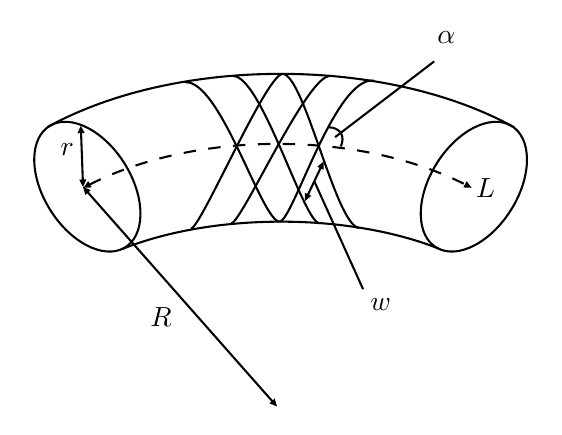
\begin{tikzpicture}[x=0.75pt,y=0.75pt,yscale=-1,xscale=1]
%uncomment if require: \path (0,310); %set diagram left start at 0, and has height of 310

%Shape: Arc [id:dp5804602983886895] 
\draw  [draw opacity=0] (83.81,74.58) .. controls (112.44,58.78) and (152.14,49) .. (196.01,49) .. controls (240.04,49) and (279.86,58.85) .. (308.51,74.74) -- (196.01,135.42) -- cycle ; \draw   (83.81,74.58) .. controls (112.44,58.78) and (152.14,49) .. (196.01,49) .. controls (240.04,49) and (279.86,58.85) .. (308.51,74.74) ;  
%Shape: Ellipse [id:dp9628309335746632] 
\draw   (85.19,73.82) .. controls (95.39,68.16) and (111.58,76.78) .. (121.36,93.09) .. controls (131.15,109.4) and (130.81,127.22) .. (120.61,132.89) .. controls (110.41,138.55) and (94.22,129.93) .. (84.44,113.62) .. controls (74.65,97.31) and (74.99,79.49) .. (85.19,73.82) -- cycle ;
%Shape: Arc [id:dp587655419756131] 
\draw  [draw opacity=0] (119.33,133.53) .. controls (139.92,125.23) and (166.79,120.21) .. (196.18,120.21) .. controls (225.14,120.21) and (251.65,125.08) .. (272.11,133.16) -- (196.18,174.7) -- cycle ; \draw   (119.33,133.53) .. controls (139.92,125.23) and (166.79,120.21) .. (196.18,120.21) .. controls (225.14,120.21) and (251.65,125.08) .. (272.11,133.16) ;  
%Shape: Ellipse [id:dp7265878739073837] 
\draw   (306.83,73.83) .. controls (317.03,79.49) and (317.37,97.31) .. (307.59,113.62) .. controls (297.81,129.93) and (281.61,138.55) .. (271.41,132.88) .. controls (261.21,127.22) and (260.87,109.4) .. (270.65,93.09) .. controls (280.43,76.78) and (296.63,68.16) .. (306.83,73.83) -- cycle ;
%Shape: Arc [id:dp4895428796944892] 
\draw  [draw opacity=0][dash pattern={on 4.5pt off 4.5pt}][line width=0.75]  (101.02,103.9) .. controls (125.21,90.81) and (158.18,82.75) .. (194.51,82.75) .. controls (230.84,82.75) and (263.81,90.81) .. (288,103.9) -- (194.51,157.88) -- cycle ; \draw [color={rgb, 255:red, 0; green, 0; blue, 0 }  ,draw opacity=1 ][dash pattern={on 4.5pt off 4.5pt}][line width=0.75]  [dash pattern={on 4.5pt off 4.5pt}]  (103.96,102.35) .. controls (127.85,90.18) and (159.63,82.75) .. (194.51,82.75) .. controls (229.57,82.75) and (261.5,90.25) .. (285.43,102.54) ; \draw [shift={(288,103.9)}, rotate = 208.42] [fill={rgb, 255:red, 0; green, 0; blue, 0 }  ,fill opacity=1 ][dash pattern={on 3.49pt off 4.5pt}][line width=0.08]  [draw opacity=0] (3.57,-1.72) -- (0,0) -- (3.57,1.72) -- cycle    ; \draw [shift={(101.02,103.9)}, rotate = 331.58] [fill={rgb, 255:red, 0; green, 0; blue, 0 }  ,fill opacity=1 ][dash pattern={on 3.49pt off 4.5pt}][line width=0.08]  [draw opacity=0] (3.57,-1.72) -- (0,0) -- (3.57,1.72) -- cycle    ;
%Straight Lines [id:da5492239734544921] 
\draw    (192.26,207) -- (102.82,105.74) ;
\draw [shift={(100.83,103.49)}, rotate = 48.54] [fill={rgb, 255:red, 0; green, 0; blue, 0 }  ][line width=0.08]  [draw opacity=0] (3.57,-1.72) -- (0,0) -- (3.57,1.72) -- cycle    ;
\draw [shift={(194.25,209.25)}, rotate = 228.54] [fill={rgb, 255:red, 0; green, 0; blue, 0 }  ][line width=0.08]  [draw opacity=0] (3.57,-1.72) -- (0,0) -- (3.57,1.72) -- cycle    ;
%Straight Lines [id:da5192811297143909] 
\draw    (100.72,100.5) -- (99.86,77) ;
\draw [shift={(99.75,74)}, rotate = 87.9] [fill={rgb, 255:red, 0; green, 0; blue, 0 }  ][line width=0.08]  [draw opacity=0] (3.57,-1.72) -- (0,0) -- (3.57,1.72) -- cycle    ;
\draw [shift={(100.83,103.49)}, rotate = 267.9] [fill={rgb, 255:red, 0; green, 0; blue, 0 }  ][line width=0.08]  [draw opacity=0] (3.57,-1.72) -- (0,0) -- (3.57,1.72) -- cycle    ;
%Curve Lines [id:da016552290131481406] 
\draw    (152.75,123.5) .. controls (157,124.5) and (189,49.25) .. (197,49) ;
%Curve Lines [id:da12423062742516078] 
\draw    (195.5,120.25) .. controls (186.75,119.75) and (167,51.5) .. (149.75,53) ;
%Curve Lines [id:da23028262569339542] 
\draw    (195.5,120.25) .. controls (202,119.75) and (222.25,50) .. (241,52.25) ;
%Curve Lines [id:da06044571228761875] 
\draw    (233.75,123.25) .. controls (222.5,121.75) and (207.5,49.5) .. (197,49) ;
%Curve Lines [id:da9064161081911803] 
\draw    (214.75,121) .. controls (207,120.5) and (186.75,49.75) .. (173,50) ;
%Curve Lines [id:da2267241249534162] 
\draw    (172.25,121) .. controls (177.25,120.75) and (209,49) .. (220,50) ;
%Shape: Arc [id:dp1346466415883305] 
\draw  [draw opacity=0] (219.16,74.75) .. controls (221.76,74.81) and (223.91,75.74) .. (225.04,77.52) .. controls (226.17,79.31) and (226.08,81.63) .. (225.01,83.99) -- (214.05,84.4) -- cycle ; \draw   (219.16,74.75) .. controls (221.76,74.81) and (223.91,75.74) .. (225.04,77.52) .. controls (226.17,79.31) and (226.08,81.63) .. (225.01,83.99) ;  
%Straight Lines [id:da5565482685396763] 
\draw    (270,43) -- (222.25,79.5) ;
%Straight Lines [id:da44756033066214673] 
\draw    (209.03,107.54) -- (215.47,93.96) ;
\draw [shift={(216.75,91.25)}, rotate = 115.35] [fill={rgb, 255:red, 0; green, 0; blue, 0 }  ][line width=0.08]  [draw opacity=0] (3.57,-1.72) -- (0,0) -- (3.57,1.72) -- cycle    ;
\draw [shift={(207.75,110.25)}, rotate = 295.35] [fill={rgb, 255:red, 0; green, 0; blue, 0 }  ][line width=0.08]  [draw opacity=0] (3.57,-1.72) -- (0,0) -- (3.57,1.72) -- cycle    ;
%Straight Lines [id:da14523083056615493] 
\draw    (235.75,152.75) -- (212.25,100.75) ;


% Text Node
\draw (131.75,160.25) node [anchor=north west][inner sep=0.75pt]   [align=left] {$\displaystyle R\ $};
% Text Node
\draw (88.5,81.25) node [anchor=north west][inner sep=0.75pt]   [align=left] {$\displaystyle r\ $};
% Text Node
\draw (270,27.25) node [anchor=north west][inner sep=0.75pt]   [align=left] {$\displaystyle \alpha $};
% Text Node
\draw (288.75,97.75) node [anchor=north west][inner sep=0.75pt]   [align=left] {$\displaystyle L\ $};
% Text Node
\draw (237.75,155.75) node [anchor=north west][inner sep=0.75pt]   [align=left] {$\displaystyle w$};


\end{tikzpicture}
